\documentclass[8pt]{extarticle}
\usepackage{multicol,caption}
\usepackage[utf8]{inputenc}
\usepackage[english]{babel}
\usepackage[a4paper, landscape, margin=1cm, footskip=0.7cm]{geometry}
\usepackage{graphicx}
\usepackage{lipsum}
\usepackage{amsmath}
\usepackage{dsfont}
\usepackage{gensymb}
\usepackage{mathrsfs}
\usepackage{framed}
\usepackage{enumerate}
\usepackage{array}
\usepackage{datetime}
\usepackage{calligra}
\usepackage[dvipsnames]{xcolor}
\usepackage[titles]{tocloft}
\usepackage[sfdefault]{roboto}
\usepackage{enumitem}
\usepackage[compact]{titlesec}


\setenumerate{itemsep=0pt,topsep=0pt}
\setitemize{itemsep=0pt, topsep=0pt}

\setlength{\parskip}{0cm}
\setlength{\parindent}{0em}
%\setlength{\headsep}{0pt}
\setlength{\topskip}{0pt}
%\setlength{\topmargin}{0pt}
\setlength{\topsep}{0pt}
\setlength{\partopsep}{0pt}

%% TOC
\graphicspath{{figures/}}

\makeatletter
\newenvironment{Table}
   {\par\bigskip\noindent\minipage{\columnwidth}\centering}
   {\endminipage\par\bigskip}
\makeatother

\setlist{nolistsep}


\newenvironment{Figure}
  {\par\medskip\noindent\minipage{\linewidth}}
  {\endminipage\par\medskip}

\newenvironment{conditions}
{\par\vspace{\abovedisplayskip}\noindent\begin{tabular}{>{$}l<{$} @{${}={}$} l}}
{\end{tabular}\par\vspace{\belowdisplayskip}}

\setlength{\columnseprule}{0.2pt}
\setlength{\columnsep}{10pt}
\renewcommand{\columnseprulecolor}{\color{lightgray}}

% TOC
\setlength{\cftbeforesecskip}{-.2ex}



\begin{document}

\begin{multicols}{3}
\noindent
\large Virtual Reality
\normalsize \\
\today, \currenttime

\section{Tipologie di occhiali}
\subsection{Occhiali 3D attivi di tipo shutter}
Un sistema 3D attivo di tipo shutter (ovvero ad immagini alternate) serve per visualizzare immagini 3D stereoscopiche. Funziona in modo da presentare l'mmagine destinata all'occhio sinistro bloccando contemporaneamente la visione dell'occhio destro, quindi presentando l'immagine all'occhio destro mentre viene bloccata quella per l'occhio sinistro, e ripetendo questo processo in modo così rapido che le interruzioni non interferiscano con la percezione delle due immagini come una singola immagine 3D. Un sistema 3D attivo di tipo shutter normalmente usa lenti shutter a cristalli liquidi (anche chiamati lenti LCD 3D). Ogni lente contiene uno strato di cristallo liquido che ha la proprietà di diventare scura quendo viene applicata una tensione elettrica, rimanendo altrimenti trasparente. Le lenti sono controllate da un segnale temporizzato che consente alle lenti di oscurarsi alternativamente sopra uno dei due occhi, in sincronia con la frequenza di aggiornamanto delle immagini di un sitema video. La sincronizzazione con l'apparato di visualizzazione può essere ottenuto per mezzo di un segnale che passa attraverso un filo oppure un segnale wireless trasmesso per mezzo di un trasmettitore a infrarossi, frequenze radio, Bluetooth o ottico. I sistemi 3D attivi vengono usati per film 3D in alcuni cinema (anche se la tecnologia più diffusa nei cinema è quella a luce polarizzata). Può essere usata per visualizzare immagini 3D images su monitor di tipo CRT, plasma, LCD e altri tipi di display video.
\subsection{Occhiali 3D a luce polarizzata}
Un sistema 3D a luce polarizzata utilizza occhiali con lenti polarizzate per creare l'illusione di immagini tridimensionali filtrando la luce che raggiunge ogni occhio. Per presentare immagini stereoscopiche e film 3D, due immagini vengono proiettate sovrapposte sullo stesso schermo o sul display attraverso diversi filtri polarizzatori. Lo spettatore indossa occhiali a basso costo che contengono una coppia di diversi filtri polarizzatori. Poiché ciascun filtro lascia passare solo la luce che è polarizzata nello stesso modo e blocca la luce polarizzata nella direzione opposta, ogni occhio vede un'immagine diversa. Questa tecnica è utilizzata per produrre un effetto tridimensionale proiettando la stessa scena in entrambi gli occhi, ma raffigurata da prospettive leggermente diverse.
\subsection{Occhiali 3D ad Anaglifi}
Anaglifo 3D è il nome dato all'effetto stereoscopico 3D realizzato per mezzo della codifica dell'immagine in ciascun occhio, usando filtri di diversi colori (di solito cromaticamente opposti), di solito rosso e ciano. Le immagini 3D con anaglifi contengono due immagini diversamente colorate, una per ciascun occhio. Quando vengono visualizzate attraverso gli "occhiali anaglifi" che filtrano l'mmagine per mezzo del "codice colore" , ciascuna delle due immagini raggiunge un solo occhio, rivelando un'immagine integrata stereoscopica. La corteccia visiva del cervello crea la percezione di una scena tridimensionale. Le immagini anaglife hanno visto una recente rinascita a causa della presentazione di immagini e video su Internet, sui dischi Blu-ray, CD, e anche in stampa.

\begin{center}
    \begin{minipage}{\columnwidth}
        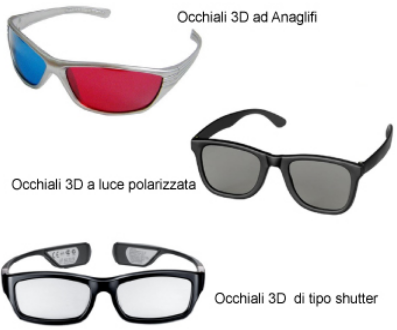
\includegraphics[width=\columnwidth]{glasses.png}
    \end{minipage}
\end{center}

\section{Powerwall}
Powerwall è un sistema meno coinvolgente di Immersive Room , ma un sistema di visualizzazione powerwall significa che un incontro può coinvolgere un gran numero di colleghi per il lavoro collaborativo. Molte persone di diversi siti possono partecipare a una determinata recensione allo stesso tempo anche se viene monitorata una sola persona. Gli schermi larghi sono ideali per visualizzare modelli di grandi dimensioni , ad esempio un grande motore.
Solitamente viene utilizzato per presentazioni o dimostrazioni VIP per scopi di vendita e marketing con partner commerciali
Revisione ingegneristica e multidisciplinare. 20.000 franchi ogni 5 metri quadrati.
\section{Cave(Cave automatic virtual Envirorment)}
Un sistema di protezione virtuale immersiva consente agli utenti di:
\begin{itemize}
    \item Analizzare i dati spazialmente correlati
    \item Concentrati sui dati con una soluzione di visualizzazione, software, calcolo e supporto completamente integrata
    \item Senti il modello 3D fluttuare nello spazio, mentre vedi le loro mani e altre persone
    \item Navigare in ambienti a grandezza naturale 
\end{itemize}
Una tipica installazione di Immersive Room include le seguenti tecnologie:
\begin{itemize}
    \item Pareti di retroproiezione
    \item Rilevamento di sensori nelle pareti
    \item Piano di proiezione giù
    \item video 
\end{itemize}
Gli utenti di Camera immersiva indossano una coppia di occhiali VR che visualizzano un'immagine 3D tramite stereoscopia . L'effetto 3D viene visualizzato visualizzando due immagini, una per occhio, che consente al cervello di interpretare la profondità degli oggetti. Con l'aiuto di un sistema di tracciamento che registra le azioni della persona all'interno di una sala immersiva, il punto di vista dell'utente è definito per visualizzare le immagini con la giusta prospettiva. 
Il costo di un sistema cave è circa di 30.000 franchi.
\subsection{Walking in the Virtual Environment}
In una cave uso una sorta di tapis roulant. 400 franchi.

\section{Motion Capture (MoCap)}
\subsection{Leap Motion e Kinect}
Il Leap è una piccola periferica USB che è stata progettata per essere posta su una scrivania reale rivolta verso l'alto. Usando 2 telecamere e 3 LED infrarossi essa osserva un'area approssimativamente a forma di semisfera di circa un metro. Essa è progettata per identificare dita (o oggetti simili come una penna) con una precisione di 0,01 mm.
Questa prodotto si differenzia dalla Kinect di Microsoft a causa dell'area di funzionamento più piccola e della migliore precisione; la kinect però è migliore da utilizzare per identificare movimenti in una stanza. In una dimostrazione al CNET viene mostrato 'The Leap' che adempie compiti come navigare in un sito web, usare il gesto pinch-to-zoom (pizzica p
er zoomare), disegno di alta precisione e manipolazione di dati in 3D. 
Leap motion 80 dollari, kinect 200 dollari.
\subsection{MYO}
Sfruttare l'attività muscolare per fornire l'input del computer presenta molti vantaggi rispetto ai dispositivi simili a Kinect che utilizzano telecamere o sensori inerziali. Un nuovo dispositivo di input wireless basato sui gesti che funziona rilevando la firma elettrica delle contrazioni degli avambracci è ora disponibile per il pre-ordine da una nuova società a \$150. La fascia da braccio, soprannominata MYO, viene fornita con un'API per sviluppatori che consente di utilizzare completamente questa sofisticata apparecchiatura.
\subsection{Marcatori passivi}
Sistemi ottici passivi che usano marcatori ricoperti da materiale retroreflettivo che riflette la luce generata da camere posizionate nell'ambiente.
Aggiustando il threshold della camera è possibile riconoscere solo parti abbaglianti ignorando il resto della scena.
Più camere vedono lo stesso marcatore e più è possibile definire in maniera precisa la sua posizione nello spazio 3D (due camere minimo).
Tale sistema implica tipicamente l'uso dalle 2 fino alle 48 camere per cui è parecchio costoso.
\subsection{Ascension Flock of Birds}
Tecnologia magnetica DC(Direct Current) pulsata per un monitoraggio dei movimenti corporei. È immune da metalli conduttivi non magnetici, è
possibile utilizzare questo tracker intorno all'acciaio inossidabile, al titanio e all'alluminio senza errori di misurazione.
\paragraph{Vantaggi}
\begin{itemize}
    \item Libertà dagli errori di blocco e occlusione.
    \item Non è necessario mantenere una linea visiva libera tra i sensori e il trasmettitore.
    \item Tracciamento simultaneo di tutti i sensori senza degrado nelle velocità di misurazione.
    \item Traccia la testa e le mani contemporaneamente senza ritardi.
    \item La copertura a lungo raggio è disponibile acquistando il trasmettitore a portata estesa (ERT / ERC).
\end{itemize}
\paragraph{Costo}
Prezzo: 1500 franchi circa
\section{Head mounted display - Augmented Reality}
\subsection{Microsoft Hololens}
Il visore si connette al proprio dispositivo mobile o ad un computer con sistema operativo Windows 10 per poter sincronizzare e avviare il dispositivo HoloLens.
Dispone di sensori di movimento, tra cui un giroscopio, un magnetometro e un accelerometro.
È acquistabile in Canada e negli Stati Uniti nella modalità di Development Edition al costo di 3000 dollari, la suite edition 5000 dollari.
L’utente può interagire principalmente con la gesture “air tap” per aprire le app, selezionare gli oggetti e spostare gli ologrammi. Grazie ai sensori che tracciano i movimenti della testa è possibile spostare il cursore con lo sguardo. Il dispositivo supporta anche i comandi vocali, quindi alcune operazioni possono essere completate con l’aiuto di Cortana.
\subsection{Google glasses}
Google Glass è una marca di smart glass, un head mounted display (HMD) che ha la forma di un paio di occhiali. I Google Glass sono stati sviluppati da X (in precedenza Google X)[1] e sono un paio di occhiali dotati di realtà aumentata, tramite i quali è possibile visualizzare informazioni come sugli smartphone senza l'uso delle mani (hands-free). I Glass si operano tramite l'uso di comandi vocali.
Il costo si aggira intorno ai 1000 dollari.

\section{Head mounted display - VR}
Un head-mounted display o HMD, è uno schermo montato sulla testa dello spettatore attraverso un casco ad hoc e può essere monoculare o binoculare.
\subsection{Samsung Gear VR}
Samsung Gear VR è un supporto per display montato come google cardboard.
Ha insieme dei controller per interfacciarsi con il mondo virtuale.
\subsection{Htc Vive}
Questo dispositivo non solo permette di vedere il mondo virtuale mediante un visore ottico, ma grazie ad una nuova tecnologia chiamata "room scale" trasforma l'ambiente che circonda l'utente in uno spazio 3D in cui può muoversi quasi liberamente. Questa nuova tecnologia associata ad un tracking della testa preciso e a dei comandi di gioco che simulano il movimento delle mani, trasforma la realtà virtuale di HTC Vive in un'esperienza particolarmente immersiva, permettendo all'utente di interagire in maniera quasi completa col mondo di gioco.
La versione PRO è dotato di display a risoluzione più elevata, ora con risoluzione 1440x1600 per-eye, insieme a una seconda fotocamera rivolta verso l'esterno, cuffie collegabili, un microfono per l'analisi dell'annullamento del rumore e un design rinnovato con una forma più "bilanciata", un peso più leggero e un quadrante di dimensionamento. Vive Pro utilizza connettori USB-C anziché USB-A. Comprende anche telecomandi che rintracciano il movimento delle mani, questi telecomandi hanno dei bottoni che servono per interfacciarsi con il mondo virtuale.
Prezzo: 499 \$
Prezzo PRO: 1098 \$
\subsection{Google Cardboard}
Google Cardboard è una piattaforma di realtà virtuale (VR) sviluppata da Google per l'uso con un supporto per indossare un head-mounted display in realtà virtuale per smartphone.  Gli utenti possono creare il proprio visore da componenti semplici e a basso costo utilizzando le specifiche pubblicate da Google oppure acquistarne uno prefabbricato. 
Prezzo: FREE o 8 CHF.
\subsection{Oculus rift}
L'Oculus Rift è il visore di realtà virtuale sviluppato da Oculus VR. Oculus Rift deve essere collegato a un computer per funzionare, un PC che deve avere una determinata potenza per gestire i giochi in realtà virtuale e i mondi virtuali proposti dagli sviluppatori. 
Può comprato con dei telecomandi chiamati Oculus Touch per detettare il movimento delle mani e per dare all’utente un modo per comunicare le proprie azioni/scelte agli utenti.
Prezzo: 399 \$
\section{Haptics}
Dispositivo VR che da un feedback tattile che può anche essere una forza opposta che non ti fa chiudere la mano quando nel mondo virtuale prendi un oggetto.
Un esempio di haptics che pero non ha la forza resistente è VR Glove chiamati Plexus che ha un feedback tattile. Prezzo 250\$.
\section{Altre tecnologie}
\subsection{Artoolkit}
ARToolKit is an open-source computer tracking library for creation of strong augmented reality applications that overlay virtual imagery on the real world.
Prezzo: 100\$

% // QUESTO E' QUELLO CHE VA INSERITO:

% DI QUESTI SOTTO POSSIAMO INSERIRE: il "giro che abbiamo fatto nel nostro progetto"
% OpenVR (stereoscopic rendering 2 p.18)
% SteamVR

% DI QUESTI SOTTO POSSIAMO INSERIRE: qualche utilizzo reale
% Skybox
% Skydome
% Object picking

% VERIFICARE E AGGIUNGERE IL MINIMO FPS:
% VR deve garantire almeno 60 frame per occhio (120 frame/secondo)

% DA AGGIUNGERE SE NON C'E' GIA' NEL LEAP MOTION:
% il leap motion può essere montato anche sopra gli headset in modo che vedi le mani nell’ambiente virtuale. Usa gli infrassossi, verificare numero camere

% CERCARE QUALCOSA SU INTERNET:
% Tuta di pura, la giacchetta (quando ti sparano)

%AGGIUNGERE:
% sensori film
% parco giochi jonny
% uforia
% aggiungere nei motion capture le tecnologie per il cinema eccetera (brief history slide 20-21)
% Dalla slide 28 alla 33 della brief history ci sono tutte le applicazioni della realtà virtuale che possiamo inserire

\end{multicols}
\end{document}
